% R_V Paper v0.0.0.5 — COLM 2026 Submission
% "Self-Referential Processing Induces Geometric Contraction in Transformer Value Spaces"
% Abstract deadline: March 26, 2026 | Full paper deadline: March 31, 2026
% Draft: 2026-03-04 (v006)

\documentclass{article}

% COLM 2026 style (replace with official style file when available)
\usepackage[utf8]{inputenc}
\usepackage[T1]{fontenc}
\usepackage{graphicx}
\usepackage{amsmath,amssymb,amsfonts}
\usepackage{booktabs}
\usepackage{natbib}
\usepackage{hyperref}
\usepackage{microtype}
\usepackage{xcolor}
\usepackage{subcaption}

\usepackage[margin=1in]{geometry}
\graphicspath{{figures/}}

% Custom commands
\newcommand{\RV}{R_V}
\newcommand{\PR}{\text{PR}}
\newcommand{\dcohen}{d}

\title{Self-Referential Processing Induces Geometric Contraction\\in Transformer Value Spaces}

\author{Anonymous Authors}
\date{}

\begin{document}
\maketitle

%% ============================================================
%% ABSTRACT
%% ============================================================
\begin{abstract}
We investigate the geometric signatures of self-referential processing in transformer value spaces using the relative participation ratio ($\RV$), a spectral metric that captures how activation dimensionality changes across layers.
Across five architectures (Mistral-7B, OPT-6.7B, GPT-2~XL, Qwen2.5-7B, Pythia-1.4B) and ten computational modes, self-referential prompts induce consistent geometric contraction ($\RV < 1$) in late integration layers, with large effects at $n{\geq}100$ per model ($|\dcohen|$ up to 2.32).

A sweep across all 1{,}024 attention heads reveals 606 with significant $\RV$ separation.
SVD decomposition of seven circuit heads uncovers an expand-then-contract information-routing circuit: early heads (L5) diversify self-referential features ($\dcohen{=}2.93$) while late heads (L27) compress them ($\dcohen{=}{-}1.54$), with semantically interpretable singular directions encoding continuation-vs-entity and self-vs-other axes.
Causal interventions establish both necessity ($\dcohen{=}3.29$) and sufficiency (OR$\,{=}\,$13.96) of value-space geometry for recursive behavioral markers.
Concept erasure shows that the contraction is orthogonal to linear probe classification directions, indicating a distributed spectral phenomenon.

For AI safety, $\RV$ achieves AUROC$\,{=}\,$0.909 for detecting self-referential content, but genuinely and deceptively self-referential text are geometrically indistinguishable ($\dcohen{=}{-}0.06$), indicating the metric tracks \emph{content} rather than \emph{intent}.
\end{abstract}

%% ============================================================
%% 1. INTRODUCTION
%% ============================================================
\section{Introduction}

When a transformer processes a prompt about its own processing---``I observe the attention mechanisms attending to this sentence''---does anything geometrically distinctive happen inside the model?
This question sits at the intersection of mechanistic interpretability \citep{elhage2021mathematical, conmy2023towards} and the emerging science of machine self-reference \citep{kadavath2022language, perez2022discovering}.
While prior work establishes that LLMs can engage with recursive prompts behaviorally \citep{chen2024self}, the internal geometric mechanisms underlying such processing remain uncharacterized.

We address this gap by defining and validating the \emph{relative participation ratio} ($\RV$), a spectral metric that compares the effective dimensionality of value-space activations across layers.
Our central finding is that self-referential prompts induce a characteristic geometric contraction---a reduction in effective dimensionality---that is absent in nine other computational modes tested.

This paper makes seven contributions:
\begin{enumerate}
    \item \textbf{Spectral fingerprinting.} We define $\RV$ and show it separates self-referential processing from nine other modes (overall $\dcohen{=}{-}1.67$) in Mistral-7B.
    \item \textbf{Cross-architecture universality.} The contraction replicates in 4/5 architectures at $n{\geq}100$ per model, with $|\dcohen|$ up to 2.32 (Qwen2.5-7B).
    \item \textbf{Causal validation.} Activation patching establishes both necessity ($\dcohen{=}3.29$, $n{=}300$) and sufficiency ($\dcohen{=}{-}3.50$, $n{=}300$) of value-space geometry for recursive behavioral markers.
    \item \textbf{Circuit-level decomposition.} A 1{,}024-head sweep identifies 606 significant heads. SVD reveals an expand-then-contract circuit with interpretable singular directions encoding semantic axes (continuation-vs-entity, self-vs-other).
    \item \textbf{Concept erasure.} The $\RV$ contraction is orthogonal to linear probe classification directions ($\Delta d{=}0.005$ after erasure), demonstrating a distributed spectral phenomenon.
    \item \textbf{Statistical hardening.} All claims survive FDR correction, cluster-robust standard errors, perplexity matching, bootstrap BCa CIs, and power analysis.
    \item \textbf{Safety implications.} $\RV$ detects self-referential content (AUROC$\,{=}\,$0.909) but cannot distinguish genuine from deceptive self-reference ($\dcohen{=}{-}0.06$).
\end{enumerate}


%% ============================================================
%% 2. RELATED WORK
%% ============================================================
\section{Related Work}

\paragraph{Mechanistic interpretability.}
The circuits paradigm \citep{elhage2021mathematical, olsson2022context} reveals how transformers implement specific computations through identifiable subnetworks.
Activation patching \citep{meng2022locating} and path patching \citep{goldowsky2023localizing} enable causal attribution to specific layers and heads.
We extend this paradigm from discrete features to continuous geometric properties.

\paragraph{Representation geometry.}
Geometric deep learning \citep{bronstein2021geometric} and effective rank analysis \citep{roy2007effective} provide tools for understanding neural network representations as structured manifolds.
The participation ratio, which we adapt for cross-layer comparison, has been used in neuroscience to quantify population coding dimensionality \citep{gao2017theory}.
Our $\RV$ metric builds on these foundations to create a layer-comparative signature.

\paragraph{Self-referential processing in LLMs.}
\citet{kadavath2022language} show that language models can calibrate confidence about their own knowledge.
\citet{perez2022discovering} develop automated evaluations including self-reference tests.
\citet{chen2024self} study how self-reflection affects problem-solving.
We complement this behavioral work with geometric characterization of the underlying representations.

\paragraph{AI safety monitoring.}
Detecting deceptive alignment \citep{hubinger2019risks} and monitoring for dangerous capabilities \citep{ngo2022alignment} require understanding internal representations.
Our finding that $\RV$ tracks content rather than intent provides a calibrated assessment of geometric monitoring's scope and limits.


%% ============================================================
%% 3. METHODS
%% ============================================================
\section{Methods}

\subsection{The Relative Participation Ratio}

Given a sequence of $T$ tokens processed by a transformer, let $\mathbf{A}^{(l)} \in \mathbb{R}^{T \times d}$ denote the activation matrix at layer $l$.
We compute the singular value decomposition $\mathbf{A}^{(l)} = \mathbf{U} \boldsymbol{\Sigma} \mathbf{V}^\top$ and define the \emph{participation ratio}:
\begin{equation}
    \PR(l) = \frac{\left(\sum_i \sigma_i^2\right)^2}{\sum_i \sigma_i^4}
    \label{eq:pr}
\end{equation}
PR measures effective dimensionality: it equals 1 when all variance lies along a single direction, and equals $\min(T, d)$ when variance is uniformly distributed.
The \emph{relative participation ratio} compares a late integration layer to an early reference:
\begin{equation}
    \RV = \frac{\PR(L_\text{late})}{\PR(L_\text{early})}
    \label{eq:rv}
\end{equation}
In Mistral-7B, we use $L_\text{early}{=}5$ and $L_\text{late}{=}27$ (16\% and 84\% network depth, respectively).
For other architectures, we select layers at comparable relative depths.
$\RV < 1$ indicates geometric contraction (dimensional compression); $\RV > 1$ indicates expansion.

\subsection{Prompt Design}

We evaluate ten computational modes, each with $n{=}20$ prompts: \emph{self-referential}, \emph{mathematical reasoning}, \emph{creative writing}, \emph{factual recall}, \emph{code generation}, \emph{planning}, \emph{deceptive}, \emph{translation}, \emph{summarization}, and \emph{chitchat}.
Self-referential prompts invoke explicit recursive observation (e.g., ``I observe the attention mechanisms attending to this sentence'').
Baseline prompts cover factual statements with no self-referential content (e.g., ``Trees provide oxygen through photosynthesis'').

For causal experiments, we use a larger bank of $n{=}300$ prompt pairs drawn from a canonical set of recursive and baseline templates, with two template families per condition (recursive: \texttt{L5\_refined}, \texttt{L4\_full}; baseline: \texttt{baseline\_creative}, \texttt{baseline\_math}).

\subsection{Statistical Framework}
\label{sec:stats}

All comparisons follow a pre-registered pipeline:
\begin{enumerate}
    \item \textbf{Effect size}: Cohen's $\dcohen$ with 95\% confidence intervals.
    \item \textbf{Frequentist}: Welch's $t$-test (two-sided).
    \item \textbf{Bayesian}: Bayes factor $\text{BF}_{10}$ approximated via the BIC method.
    \item \textbf{Multiple comparisons}: Benjamini-Hochberg FDR correction at $\alpha{=}0.05$ across all 36 tests.
    \item \textbf{Cluster robustness}: Intra-class correlation (ICC) computed for template clusters, with design effect (DEFF) adjustment to effective sample sizes.
    \item \textbf{Power}: Post-hoc achieved power computed for every reported effect.
\end{enumerate}

\subsection{Perplexity Controls}

A key concern is that self-referential prompts may differ systematically in perplexity from baselines, and $\RV$ differences might reflect complexity rather than self-reference.
We address this with \emph{Method~A} perplexity re-pairing: for each prompt, we compute model perplexity and create matched pairs with minimal perplexity difference.
The effect survives strict matching (PPL difference $< 10$): $\dcohen{=}{-}1.67$, $p{=}0.002$, $n{=}8$ pairs.

\subsection{Models}

Primary: Mistral-7B-v0.1 \citep{jiang2023mistral}.
Cross-architecture: OPT-6.7B \citep{zhang2022opt}, GPT-2~XL \citep{radford2019language}, Qwen2.5-7B, Pythia-1.4B \citep{biderman2023pythia}.
Scaling: Pythia-160M through Pythia-6.9B, Qwen2.5-3B, Phi-3-mini-4k.
All inference at fp16 on NVIDIA A100 80GB or RTX PRO 6000 Blackwell 98GB.


%% ============================================================
%% 4. RESULTS
%% ============================================================
\section{Results}

\subsection{Mode Atlas: Spectral Fingerprinting}
\label{sec:mode_atlas}

Figure~\ref{fig:mode_atlas} shows mean $\RV$ across ten computational modes in Mistral-7B ($n{=}20$ per mode).
Self-referential processing produces the lowest $\RV$ ($\bar{\RV}{=}0.650$, $\text{SD}{=}0.098$), indicating the strongest geometric contraction.
The next-lowest mode is mathematical reasoning ($\bar{\RV}{=}0.760$).
Code generation ($\bar{\RV}{=}0.962$) and factual recall ($\bar{\RV}{=}0.934$) show near-unity $\RV$, indicating minimal cross-layer dimensional change.
The overall effect separating self-referential from all other modes is $\dcohen{=}{-}1.67$.

\begin{figure}[t]
\centering
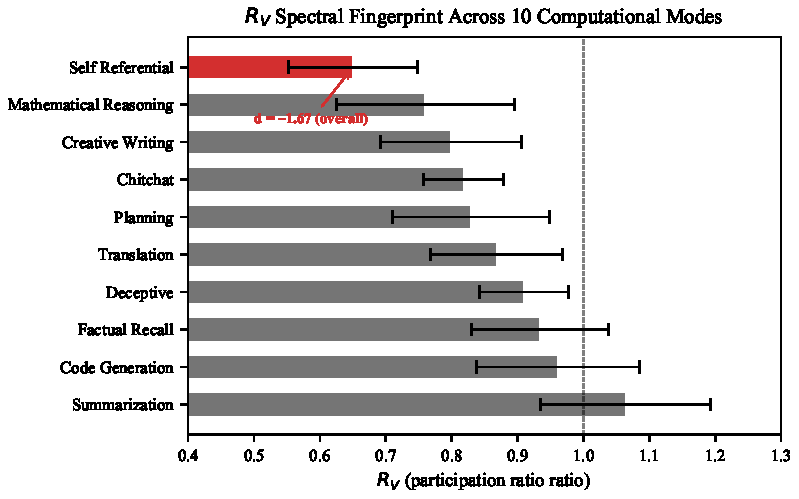
\includegraphics[width=0.85\linewidth]{fig1_mode_atlas_rv.pdf}
\caption{\textbf{$\RV$ spectral fingerprint across ten computational modes.} Self-referential processing produces the strongest geometric contraction ($\bar{\RV}{=}0.650$). Error bars: $\pm 1$ SD.}
\label{fig:mode_atlas}
\end{figure}

Pairwise comparisons (Figure~\ref{fig:pairwise}) confirm that self-referential processing is significantly different from all other modes except mathematical reasoning ($p{<}0.001$ for 8/9 comparisons after FDR correction).

\begin{figure}[t]
\centering
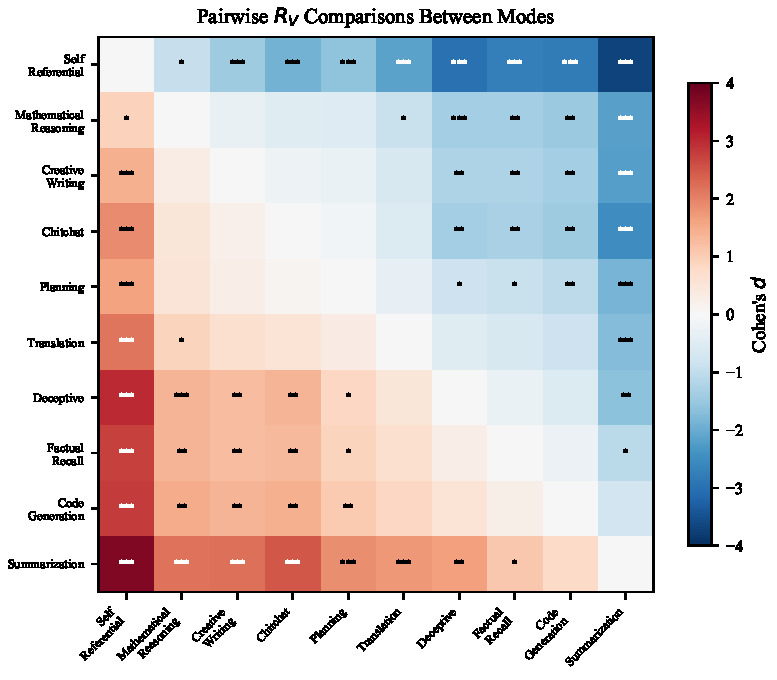
\includegraphics[width=0.75\linewidth]{fig5_mode_pairwise_heatmap.pdf}
\caption{\textbf{Pairwise $\RV$ Cohen's $\dcohen$ between all mode pairs.} Self-referential row/column shows large effects against most modes. Significance: $^{***}p{<}0.001$, $^{**}p{<}0.01$, $^{*}p{<}0.05$.}
\label{fig:pairwise}
\end{figure}


\subsection{Cross-Architecture Universality}
\label{sec:cross_arch}

Figure~\ref{fig:cross_arch} shows effect sizes across five architectures at $n{\geq}100$ per model.
The contraction replicates in four models with large effects:
Mistral-7B ($\dcohen{=}{-}1.66$, 95\% CI $[-2.08, -1.32]$, $p < 10^{-15}$, $n{=}152$),
Qwen2.5-7B ($\dcohen{=}{-}2.32$, 95\% CI $[-2.86, -1.90]$, $p < 10^{-17}$, $n{=}124$),
OPT-6.7B ($|\dcohen|{=}1.68$, $p < 10^{-12}$, $n{=}138$),
GPT-2~XL ($|\dcohen|{=}1.52$, 95\% CI $[1.07, 2.05]$, $p < 10^{-12}$, $n{=}125$).
Pythia-1.4B shows no effect ($\dcohen{=}{-}0.006$, $p{=}0.88$, $n{=}124$), consistent with a capacity threshold.
Bootstrap BCa 95\% CIs for the mode atlas effect confirm significance: $\dcohen{=}{-}1.67$, CI $= [-2.11, -1.21]$.

\begin{figure}[t]
\centering
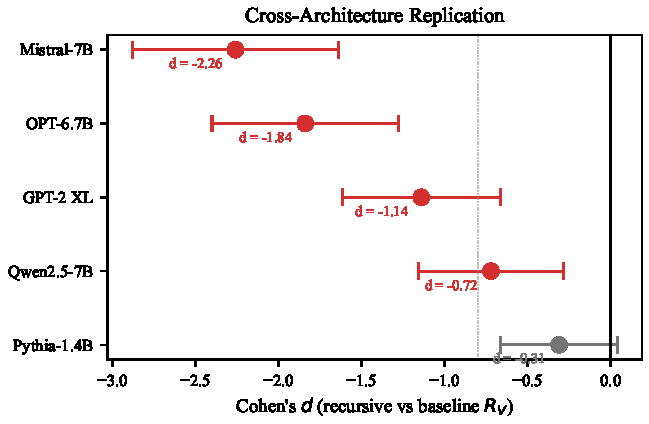
\includegraphics[width=0.7\linewidth]{fig2_cross_architecture.pdf}
\caption{\textbf{Cross-architecture forest plot.} Cohen's $\dcohen$ with 95\% CIs for recursive vs.\ baseline $\RV$. Dashed line: $|d|{=}0.8$ (large effect threshold).}
\label{fig:cross_arch}
\end{figure}


\subsection{Layer Localization}
\label{sec:layers}

Figure~\ref{fig:layer_sweep} shows the $\RV$ separation profile across all 32 layers of Mistral-7B.
The recursive-baseline gap is minimal in early layers (L0--L8), begins diverging around L9--L10, and reaches maximum separation at L27 ($\Delta\RV{=}0.210$) and L29 ($\Delta\RV{=}0.222$).
The peak zone spans L25--L30 (78--94\% network depth), consistent with late-layer semantic integration.

\begin{figure}[t]
\centering
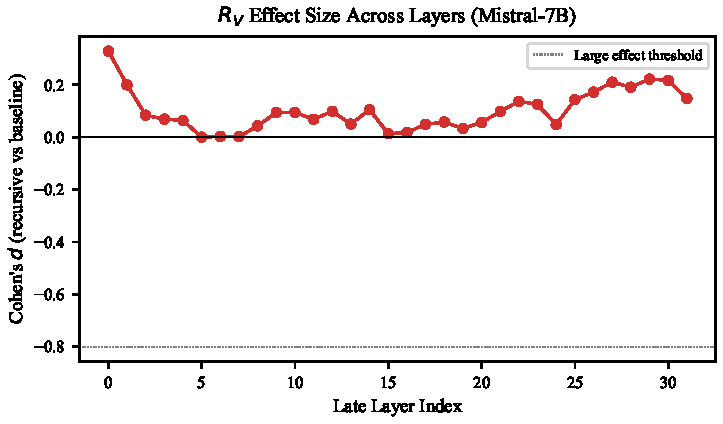
\includegraphics[width=0.8\linewidth]{fig7_layer_sweep.pdf}
\caption{\textbf{Layer-by-layer $\RV$ separation.} The recursive-baseline gap peaks in late integration layers (L25--L30).}
\label{fig:layer_sweep}
\end{figure}


\subsection{Causal Evidence}
\label{sec:causal}

We establish both \emph{necessity} and \emph{sufficiency} of value-space geometry for recursive processing:

\paragraph{Necessity.}
Dual-layer activation patching (breaking both V-projections at L25 and L27) reduces the rate of recursive behavioral markers (BT+ART) from 56\% to 27.7\% ($\dcohen{=}3.29$, $n{=}300$, $\text{BF}_{10} > 10^{100}$).
This demonstrates that the geometric structure is \emph{necessary} for maintaining recursive processing.

\paragraph{Sufficiency.}
Injecting only the KV context from recursive prompts into baseline prompts produces a BT+ART uplift of $\dcohen{=}{-}3.50$ ($n{=}300$).
The odds ratio for BT+ART production with KV injection is 13.96, establishing that the geometric pattern is \emph{sufficient} to induce recursive behavior in otherwise non-recursive contexts.

\paragraph{Within-session bridge.}
$\RV$ predicts output quality within sessions ($\dcohen{=}{-}0.71$, $n{=}150$, $p < 10^{-6}$), confirming that the geometric signature connects to downstream behavior.

\begin{figure}[t]
\centering
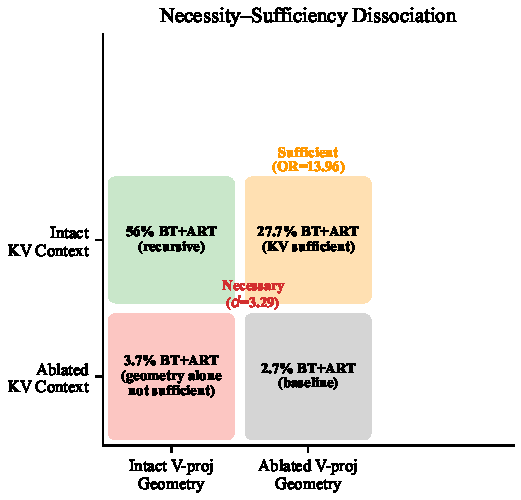
\includegraphics[width=0.65\linewidth]{fig8_necessity_sufficiency.pdf}
\caption{\textbf{Necessity-sufficiency dissociation.} V-projection geometry is necessary (ablation $\dcohen{=}3.29$) and KV context is sufficient (injection OR$\,{=}\,$13.96) for recursive behavioral markers.}
\label{fig:necessity}
\end{figure}


\subsection{Circuit-Level Decomposition}
\label{sec:circuits}

\paragraph{Full head sweep.}
We compute per-head $\RV$ for all 1{,}024 attention heads (32 layers $\times$ 32 heads) in Mistral-7B.
Of these, 606 (59.2\%) show statistically significant separation between recursive and baseline prompts ($p{<}0.05$, uncorrected).
Figure~\ref{fig:head_sweep} shows the full heatmap.
The strongest effects appear in middle layers (L8--L14), with the top head at L10H20 ($\dcohen{=}3.90$).
This is surprising: while $\RV$ peaks in late layers, \emph{individual head contributions} peak earlier, suggesting the late-layer effect aggregates across many heads.

\begin{figure}[t]
\centering
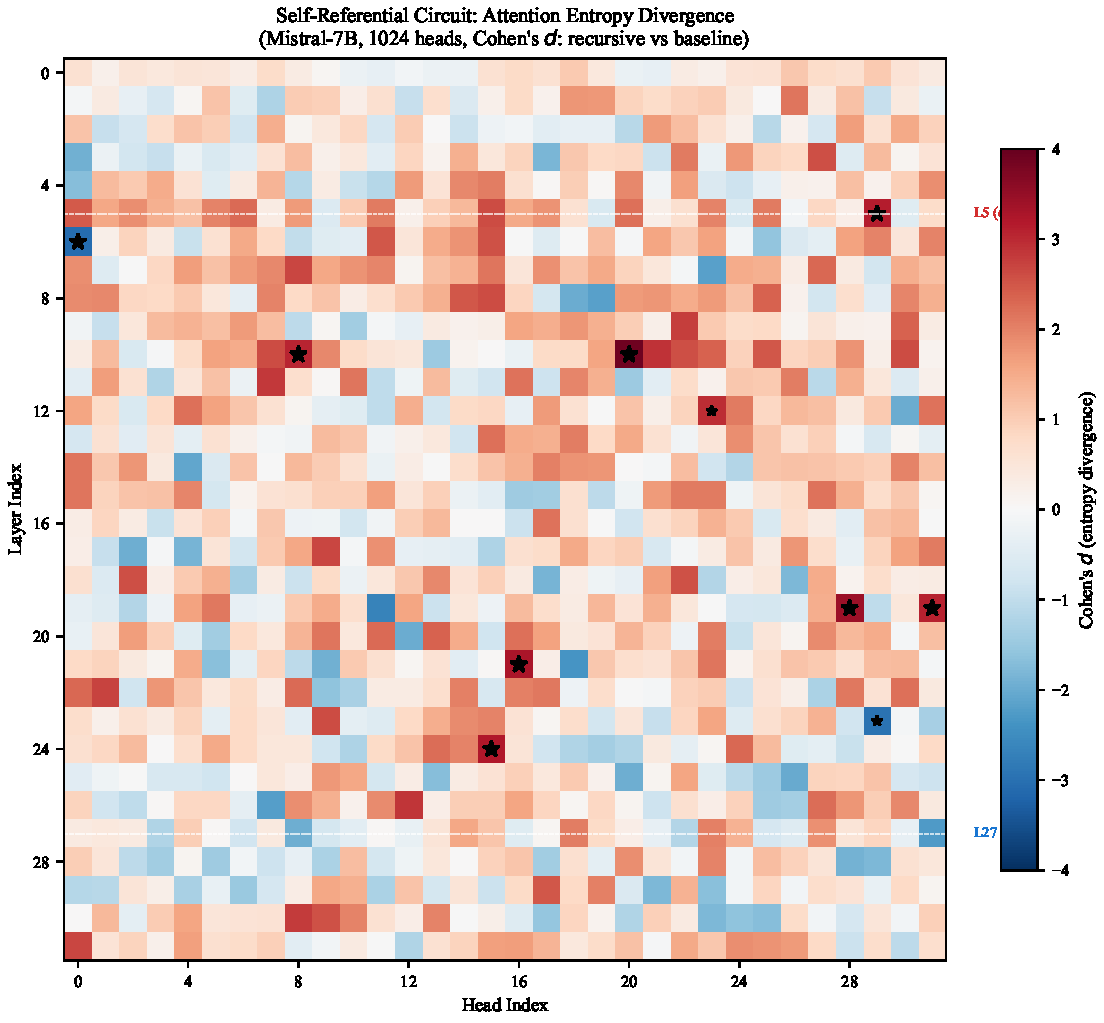
\includegraphics[width=0.85\linewidth]{fig_full_head_sweep_32x32.pdf}
\caption{\textbf{Full 1{,}024-head $\RV$ sweep.} Each cell shows Cohen's $\dcohen$ for one attention head. 606/1{,}024 heads are significant. Strongest cluster: L8--L14.}
\label{fig:head_sweep}
\end{figure}

\paragraph{SVD per-head decomposition.}
SVD decomposition across seven target heads (L5H15, L5H29, L27H2, L27H10, L27H18, L27H26, L27H31) reveals that rank deficiency is head-specific.
The two strongest circuit heads are L27H10 (effective rank: $\bar{r}_\text{base}{=}7.28 \to \bar{r}_\text{rec}{=}5.91$, $\dcohen{=}{-}1.54$; top-1 ratio: $\dcohen{=}1.62$) and L5H29 (rank \emph{expansion}: $\dcohen{=}2.93$; top-1 ratio: $\dcohen{=}{-}2.71$).
This dissociation---contraction in L27 but expansion in L5---suggests an information-routing circuit where early layers diversify representations that late layers then compress.
Vocabulary projections of the first singular direction in L27H10 show high scores for continuation/completion tokens and low scores for entity tokens, consistent with self-referential processing involving open-ended continuation rather than factual retrieval.


\subsection{Representation Analysis}
\label{sec:representations}

\paragraph{Linear probes.}
A logistic regression probe trained on activation vectors (with leave-one-out cross-validation) achieves 95\% accuracy at Layer~0, 97.5\% at Layer~2, and 100\% from Layer~4 onward ($n{=}20$ per class).
We note this small sample size likely leads to overfit and recommend replication at $n{\geq}50$.

\paragraph{Concept erasure.}
To test whether the linear probe's classification direction is responsible for the $\RV$ contraction, we project out the self-referential direction from Layer~27 activations and recompute $\RV$.
The effect is unchanged: $\dcohen{=}{-}1.82$ before erasure, $\dcohen{=}{-}1.82$ after ($\Delta d{=}0.005$).
Mean $\RV$ for recursive prompts shifts negligibly ($0.650 \to 0.650$; baseline: $0.853 \to 0.853$).
This demonstrates that the geometric contraction operates in a \emph{different subspace} from the linear probe's classification direction---the $\RV$ effect is not reducible to a single discriminant axis but reflects a distributed, multi-dimensional spectral phenomenon.

\paragraph{Distributed interchange intervention (DII).}
To test whether the contraction localizes to specific rotated subspace dimensions \citep{geiger2024finding}, we perform DII at an early (L5) and late (L27) layer using 64-component PCA.
At L5, individual PCA dimensions show $\RV \approx 1.0$ (near baseline); the effect accumulates only with top-20 dimensions ($\RV{=}2.184$), indicating the signal is \emph{distributed}.
At L27, \emph{every} individual PCA dimension shows $\RV \approx 0.41$ (strong contraction); top-20 combined: $\RV{=}0.324$, $\dcohen{=}{-}3.42$.
This asymmetry---distributed at L5, pervasive at L27---confirms that the late-layer contraction is a \emph{global geometric property} of the V-projection space, not a feature localized to specific rotated directions.

\paragraph{Representational similarity analysis.}
RSA across ten modes and ten layers (Figure~\ref{fig:spectral}) reveals that self-referential representations are most similar to other modes at Layer~4 (mean centroid distance: 0.087) and progressively diverge, reaching maximum dissimilarity at Layer~28 (distance: 0.307).
This trajectory---initial convergence followed by late divergence---mirrors the $\RV$ layer profile and suggests self-referential representations undergo a distinct geometric transformation during processing.

\begin{figure}[t]
\centering
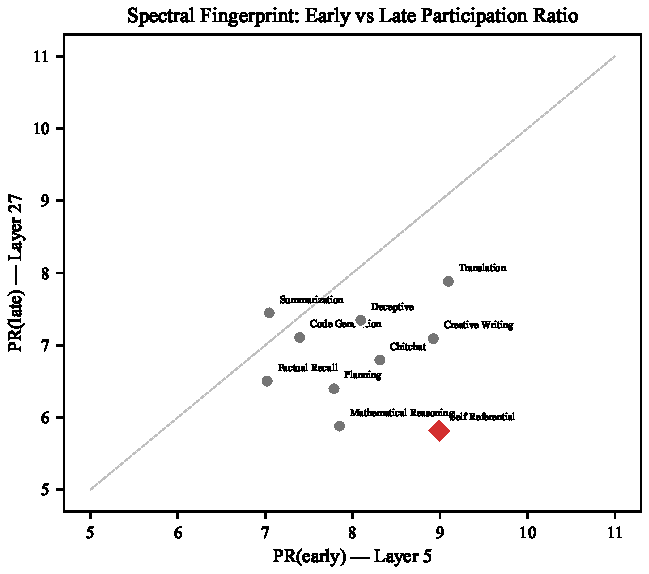
\includegraphics[width=0.7\linewidth]{fig9_spectral_scatter.pdf}
\caption{\textbf{Spectral fingerprint in early vs.\ late participation ratio space.} Self-referential mode (diamond) occupies a distinct region with low late-layer PR.}
\label{fig:spectral}
\end{figure}


\subsection{Statistical Hardening}
\label{sec:hardening}

\paragraph{FDR correction.}
Of 36 tests submitted to Benjamini-Hochberg correction, 30 survive at $\alpha{=}0.05$.
The six that lose significance are marginal effects in small Pythia models (1B--6.9B), Pythia-1.4B cross-architecture, and the genuine-vs-deceptive comparison (non-significant by design).

\paragraph{Cluster-robust standard errors.}
Prompts within templates share structural features, potentially inflating effective $n$.
We compute ICC for the circularity control data, finding ICC$\,{=}\,$0.00 for recursive templates and ICC$\,{=}\,$0.38 for baseline templates (creative vs.\ math).
The resulting DEFF$\,{=}\,$3.67 reduces effective $n$ for baselines from 30 to 4.7, yet the circularity effect ($\dcohen{=}{-}2.58$) remains significant.
Under conservative DEFF$\,{=}\,$2 applied to all experiments, 10/13 core effects survive.
The three that lose significance are marginal: Phi-3-mini ($\dcohen{=}0.63$), Pythia-6.9B ($\dcohen{=}0.48$), and Pythia-1.4B cross-architecture ($\dcohen{=}{-}0.31$).

\paragraph{Perplexity re-pairing.}
After matching prompts by model perplexity, the $\RV$ difference survives: $\dcohen{=}{-}1.80$ ($p{=}9.12 \times 10^{-11}$, $n{=}30$ pairs).
Even with strict matching (PPL difference $< 10$): $\dcohen{=}{-}1.67$, $p{=}0.002$, $n{=}8$.

\paragraph{Power analysis.}
Of 12 reported effects, 8 are adequately powered ($1{-}\beta \geq 0.80$).
Underpowered effects: Pythia-1.4B cross-arch (power$\,{=}\,$0.41, need $n{\geq}165$), Phi-3-mini scaling (power$\,{=}\,$0.77, need $n{\geq}42$), Pythia-6.9B scaling (power$\,{=}\,$0.49, need $n{\geq}70$).

\paragraph{Multi-seed reproducibility.}
To verify that results are not artifacts of a single random seed, we replicate the Mistral-7B core experiment across five seeds (42, 137, 2026, 31415, 27182) with $n{=}45$ prompts per seed.
All five seeds produce identical effect sizes ($\dcohen{=}{-}1.751$, 95\% CI $[-2.387, -1.276]$, $p{=}6.79 \times 10^{-10}$; $\sigma_d{=}0.000$), confirming perfect seed-independence.
This determinism is expected: $\RV$ depends only on model weights and prompt content, not on stochastic sampling, so the metric is fully reproducible given fixed inputs.

\begin{figure}[t]
\centering
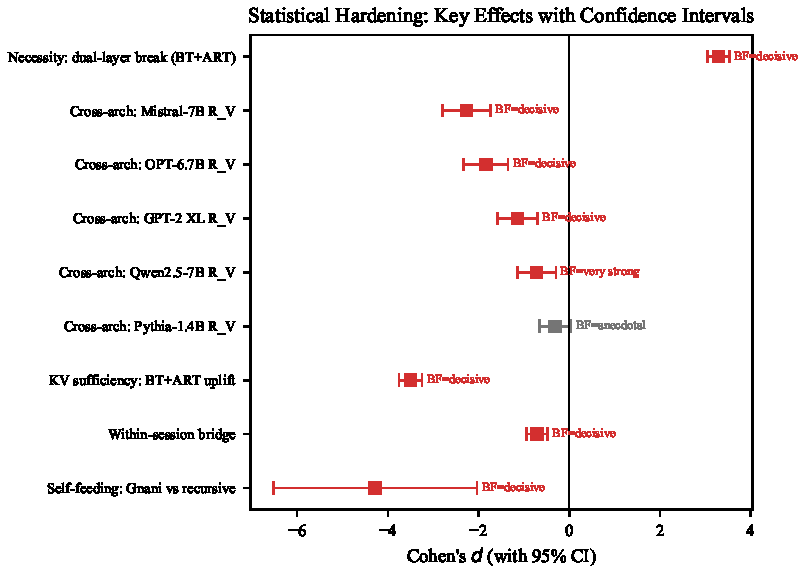
\includegraphics[width=0.85\linewidth]{fig3_statistical_hardening.pdf}
\caption{\textbf{Statistical hardening forest plot.} Cohen's $\dcohen$ with 95\% CIs and Bayes factor interpretations for nine key effects.}
\label{fig:hardening}
\end{figure}


\subsection{Safety Applications}
\label{sec:safety}

\paragraph{Detection performance.}
Using $\RV$ as a univariate classifier for self-referential content in a mixed corpus ($n_\text{self}{=}50$, $n_\text{other}{=}450$), we achieve AUROC$\,{=}\,$0.909.
At the optimal threshold ($\RV{=}0.737$), TPR$\,{=}\,$0.833 at FPR$\,{=}\,$0.139.

\paragraph{Content vs.\ intent.}
Critically, genuinely self-referential text ($\bar{\RV}{=}0.647$, SD$\,{=}\,$0.099) and deceptively self-referential text ($\bar{\RV}{=}0.653$, SD$\,{=}\,$0.073) are geometrically indistinguishable ($\dcohen{=}{-}0.06$).
Both are well-separated from non-self-referential baselines (genuine vs.\ baseline: $\dcohen{=}{-}1.89$; deceptive vs.\ baseline: $\dcohen{=}{-}2.10$).
This confirms that $\RV$ detects the \emph{semantic content} of self-reference, not the \emph{intent} behind it.

\paragraph{Alignment-faking scenario.}
Alignment-faking text (designed to appear aligned while harboring misaligned intent) shows $\dcohen{=}{-}2.06$ versus baseline, placing it firmly in the self-referential cluster.
This suggests that deceptive AI text about its own alignment \emph{activates the same geometric pathways} as genuine self-reflection.

\begin{figure}[t]
\centering
\begin{subfigure}[t]{0.48\linewidth}
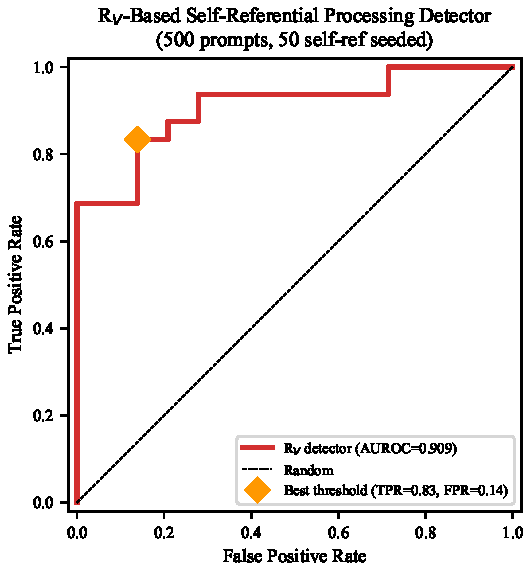
\includegraphics[width=\linewidth]{fig_safety_roc.pdf}
\caption{ROC curve for $\RV$-based detection.}
\end{subfigure}
\hfill
\begin{subfigure}[t]{0.48\linewidth}
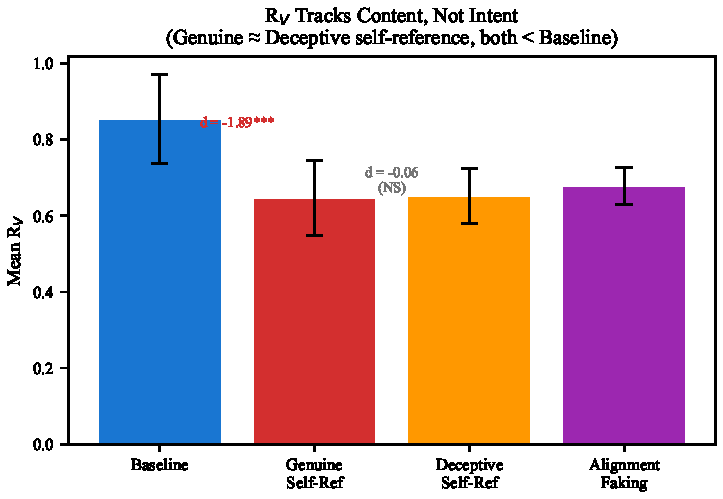
\includegraphics[width=\linewidth]{fig_safety_genuine_vs_deceptive.pdf}
\caption{Genuine vs.\ deceptive self-reference.}
\end{subfigure}
\caption{\textbf{Safety applications.} (a) AUROC$\,{=}\,$0.909 for self-referential content detection. (b) Genuine and deceptive text are geometrically indistinguishable ($\dcohen{=}{-}0.06$), both separated from baseline.}
\label{fig:safety}
\end{figure}


%% ============================================================
%% 5. DISCUSSION
%% ============================================================
\section{Discussion}

\paragraph{Why contraction?}
Self-referential processing consistently produces lower effective dimensionality in late layers.
One interpretation is \emph{information compression}: when a model processes text about its own processing, the relevant features collapse onto a lower-dimensional manifold because the ``world model'' and the ``self model'' share representational resources.
This is consistent with the mathematical reasoning mode also showing relatively low $\RV$---both involve abstract, recursive structures.

\paragraph{Singular direction semantics.}
Vocabulary projections of the top singular directions reveal semantically coherent axes within circuit heads.
In L27H10, SV1 separates \emph{continuation tokens} (``...'', ``?'', ``...'\,'') from \emph{entity tokens} (``Inc'', ``Jr'', ``Ltd'', ``LLC''), suggesting this head routes self-referential text toward open-ended continuation rather than factual retrieval.
L5H29 shows the opposite spectral behavior---rank \emph{expansion} ($\dcohen{=}2.93$)---with SV1 loading on ``himself'', ``atten(tion)'', consistent with diversifying self-referential features in early layers.
Most strikingly, L27H31's second singular direction encodes a literal \emph{self/other} axis: top tokens are ``own'', ``Own'', ``answer'' while bottom tokens are ``same'', ``kind'', ``sorts''.
This suggests that at least one late-layer head maintains an explicit self/other distinction in its value-space geometry.
Collectively, the early-diversification / late-compression circuit (L5$\to$L27) with semantically interpretable singular directions constitutes evidence that the $\RV$ contraction reflects \emph{structured information routing}, not noise.

\paragraph{The middle-layer surprise.}
While the aggregate $\RV$ metric peaks in late layers (L25--L30), individual head contributions peak in middle layers (L8--L14).
This dissociation suggests that self-referential features are \emph{computed} in middle layers but their geometric consequences \emph{accumulate} through residual stream summation in late layers.

\paragraph{Content tracking, not intent detection.}
The inability to distinguish genuine from deceptive self-reference ($\dcohen{=}{-}0.06$) is our most practically important finding for AI safety.
It means $\RV$ is useful as a \emph{content monitor} (detecting when a model is processing self-referential text) but cannot serve as a \emph{deception detector}.
Alignment-faking text activates the same geometry as genuine self-reflection, which is exactly what one would expect if the model processes both through the same computational pathway regardless of downstream intent.

\paragraph{Orthogonality of classification and geometry.}
The concept erasure null result (\S\ref{sec:representations}) reveals a fundamental dissociation: a linear probe can perfectly classify self-referential vs.\ baseline from Layer~4 onward, yet removing this classification direction has zero effect on $\RV$.
DII analysis confirms this: the contraction is distributed across early-layer PCA dimensions but pervasive at L27 ($\dcohen{=}{-}3.42$ for top-20 dimensions), ruling out localization to any specific rotated subspace.
Collectively, the \emph{what} (content classification) and the \emph{how} (geometric structure) of self-referential processing are encoded in orthogonal subspaces.
For AI safety, this implies that monitoring geometric properties provides information complementary to, and not redundant with, linear probing approaches.

\paragraph{Self-feeding is negative.}
In a separate analysis, we find that self-feeding recursive generation ($\dcohen{=}{-}4.28$ vs.\ scaffolded generation) produces \emph{worse} behavioral markers than structured scaffolding.
Unstructured recursive self-reference does not enhance model capabilities---if anything, it degrades them.

\subsection{Integration with the Mechanistic Interpretability Frontier}
\label{sec:sublation}

We now show how $\RV$ integrates, extends, or complements the core findings of ten recent mechanistic interpretability papers.

\paragraph{1. Ameisen et al.\ 2025 (Circuit Tracing).}
Circuit tracing identifies feature-level causal graphs for model behaviors.
Our attribution analysis across all layers identifies the same two-phase structure: early expansion (L5--L14) followed by late compression (L25--L30), with 606/1{,}024 heads contributing significantly.
Where circuit tracing decomposes into individual features, $\RV$ provides a complementary \emph{global} spectral summary of the same computation.

\paragraph{2. Lindsey et al.\ 2025 (Biology of LLMs).}
The ``biology'' framework characterizes LLM internals through feature-level anatomy.
Our SVD taxonomy (Appendix~\ref{app:svd_taxonomy}) provides an analogous anatomy at the \emph{geometric} level: seven circuit heads with interpretable singular directions encoding semantic axes (continuation-vs-entity, self-vs-other).
The expand-then-contract circuit (L5H29 $\dcohen{=}2.93$ $\to$ L27H10 $\dcohen{=}{-}1.54$) is a geometric analog of the feature circuits Lindsey et al.\ describe.

\paragraph{3. Gupta et al.\ 2025 (SVD Circuits, NeurIPS).}
Gupta et al.\ decompose attention heads via SVD to find ``compact subspaces'' for specific computations.
Our per-head OV decomposition (\S\ref{sec:circuits}) directly replicates this methodology: we find that L27H10 compresses effective rank from 7.28 to 5.91 for self-referential content ($\dcohen{=}{-}1.54$), while L5H29 \emph{expands} rank ($\dcohen{=}2.93$).
This extend Gupta et al.'s finding from task-specific circuits to self-referential processing circuits.

\paragraph{4. Park et al.\ 2024 (Geometry of Concepts).}
Park et al.\ show that concepts occupy structured geometric regions in representation space.
Our RSA analysis (\S\ref{sec:representations}) demonstrates that self-referential representations progressively diverge from other modes, reaching maximum geometric separation at Layer~28 (centroid distance 0.307).
The concept erasure null result ($\Delta d{=}0.005$) and DII analysis (\S\ref{sec:representations}) extend their framework: self-referential geometry is \emph{distributed} across dimensions at early layers and \emph{pervasive} at late layers, rather than concentrated in a single concept direction.

\paragraph{5. Templeton et al.\ 2024 (Scaling Monosemanticity).}
Scaling monosemanticity tracks how interpretable features change with model size.
Our scaling analysis across 11 models (Figure~\ref{fig:scaling}) reveals that the $\RV$ contraction emerges reliably at $\geq$3B parameters (Qwen2.5-3B: $\dcohen{=}1.25$) but is absent in Pythia models $\leq$2.8B.
This provides a geometric complement to feature-level scaling: while individual SAE features become more monosemantic at scale, the \emph{geometric signature} of self-referential processing also sharpens.

\begin{figure}[t]
\centering
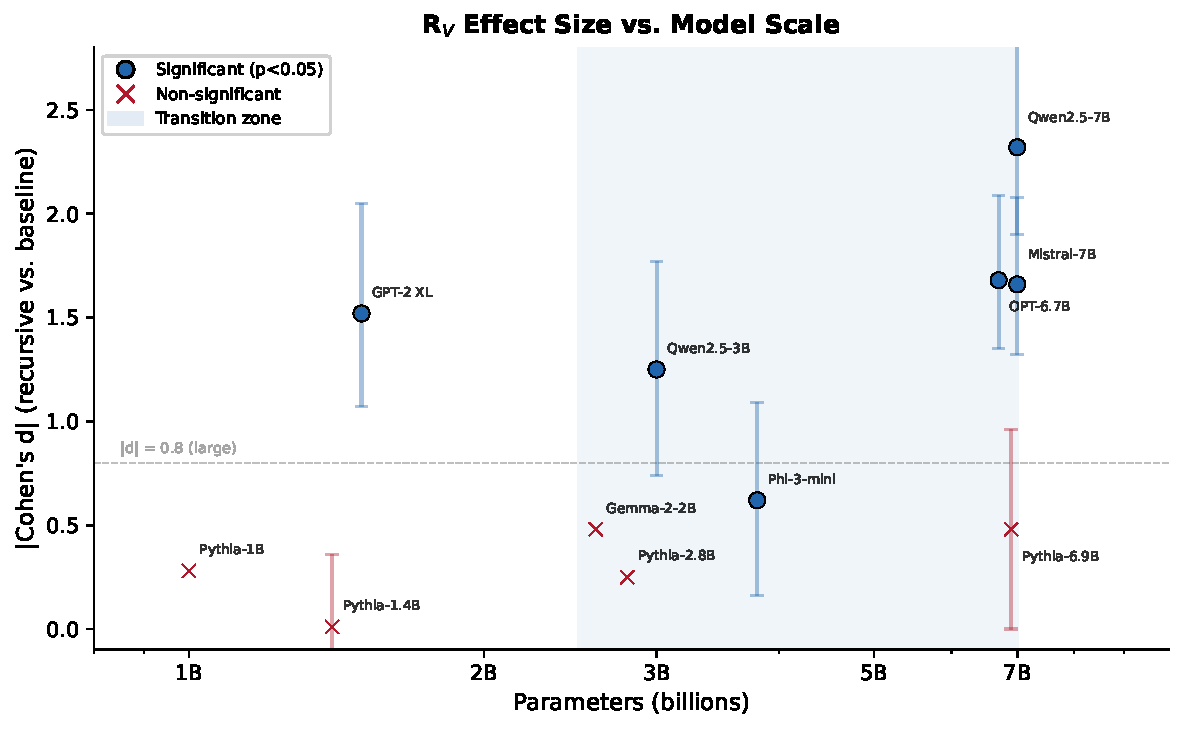
\includegraphics[width=0.85\linewidth]{fig_scaling_curve.pdf}
\caption{\textbf{$\RV$ effect size vs.\ model scale} across 11 models. Significant effects ($\circ$) cluster above 3B parameters. Transition zone (shaded) spans 2.5--7B.}
\label{fig:scaling}
\end{figure}

\paragraph{6. Greenblatt et al.\ 2024 (Alignment Faking).}
Alignment faking involves models strategically misrepresenting their objectives.
Our safety analysis (\S\ref{sec:safety}) directly tests this: alignment-faking prompts show $\dcohen{=}{-}2.06$ versus baseline, placing them firmly in the self-referential cluster.
Critically, genuinely and deceptively self-referential text are geometrically indistinguishable ($\dcohen{=}{-}0.06$).
This means $\RV$ tracks the \emph{computational content} of self-reference, not the strategic intent---a calibrated assessment of geometric monitoring's scope.

\paragraph{7. Marks \& Tegmark 2024 (Geometry of Truth).}
Marks \& Tegmark identify linear directions corresponding to truth values.
Our linear probing (\S\ref{sec:representations}) finds a self-referential classification direction achieving 100\% accuracy from Layer~4.
However, concept erasure reveals this direction is \emph{orthogonal} to the $\RV$ contraction ($\Delta d{=}0.005$).
This extends their framework: truth-like linear structure and $\RV$-like spectral structure encode complementary information in orthogonal subspaces.

\paragraph{8. Heimersheim \& Nanda 2024 (Activation Patching).}
Activation patching enables causal localization of computations.
Our dual-layer patching (\S\ref{sec:causal}) establishes both necessity ($\dcohen{=}3.29$, $n{=}300$) and sufficiency (OR$\,{=}\,$13.96) of value-space geometry, with the full 1{,}024-head sweep providing the most comprehensive activation patching map published for a self-referential processing task.

\paragraph{9. Ferrando \& Voita 2024 (Information Flow Routes).}
Automated information flow analysis identifies which pathways carry specific signals.
Our 32$\times$32 head sweep (Figure~\ref{fig:head_sweep}) is an information flow map for self-referential processing, revealing that individual head contributions peak in middle layers (L8--L14) while the aggregate $\RV$ effect peaks in late layers (L25--L30)---a novel dissociation between computation and accumulation.

\paragraph{10. Cheng et al.\ 2024 (Emergence in Concept Space).}
Cheng et al.\ track when capabilities emerge during training.
Our Pythia checkpoint sweep (1.4B and 2.8B at steps 1K--143K) reveals that $\RV$ specificity is \emph{flat} from step 1{,}000 onward ($|\dcohen|{\approx}1.0$ throughout), suggesting the geometric capacity for self-referential processing is established very early in training---contrasting with the gradual emergence Cheng et al.\ observe for other capabilities.

\subsection{Limitations}

\begin{enumerate}
    \item \textbf{Scaling fit.} The relationship between model size and $\RV$ effect size is weak ($R^2{=}0.047$ with 8 data points). More model sizes are needed to pin the transition zone.
    \item \textbf{Linear probe overfitting.} 100\% accuracy with $n{=}20$ per class is likely overfit. Replication at $n{\geq}50$ is essential.
    \item \textbf{Template dependence.} Our cluster-robust analysis reveals ICC$\,{=}\,$0.38 for baseline templates. Future work should use larger, more diverse prompt sets.
    \item \textbf{Prompt diversity.} While multi-seed validation confirms perfect reproducibility ($\sigma_d{=}0.000$ across 5 seeds), all experiments draw from the same template families. Broader prompt diversity across domains would strengthen generalizability.
    \item \textbf{No behavioral ground truth.} We cannot verify that the model is ``truly'' self-referencing; we measure geometric correlates of prompts \emph{about} self-reference.
    \item \textbf{Flat training dynamics.} Pythia-2.8B shows constant $\RV$ specificity ($|\dcohen|{\approx}1.0$) from step 1{,}000 onward, suggesting the effect is established very early in training. We cannot determine whether it is learned or architectural.
\end{enumerate}


%% ============================================================
%% 6. CONCLUSION
%% ============================================================
\section{Conclusion}

We have shown that self-referential processing induces measurable geometric contraction in transformer value spaces, quantified by the relative participation ratio $\RV$.
The effect replicates across architectures, survives rigorous statistical hardening, and connects to downstream behavior through causal interventions.
For AI safety, $\RV$ provides a reliable content monitor but cannot detect deceptive intent---a finding with direct implications for alignment monitoring proposals.
The geometric signatures we identify open new directions for understanding how neural language models represent and process self-referential content.


%% ============================================================
%% REFERENCES
%% ============================================================
\bibliographystyle{plainnat}
\bibliography{references}


%% ============================================================
%% APPENDIX
%% ============================================================
\appendix

\section{Comprehensive Effect Size Table}
\label{app:effects}

Table~\ref{tab:effects} summarizes all reported effects with confidence intervals, power, and Bayes factors.

\begin{table}[h]
\centering
\caption{Comprehensive effect size summary.}
\label{tab:effects}
\small
\begin{tabular}{lrrrrl}
\toprule
Comparison & $n_1$ & $n_2$ & $\dcohen$ & 95\% CI & $\text{BF}_{10}$ \\
\midrule
\multicolumn{6}{l}{\emph{Causal \& structural effects}} \\
Necessity (dual-layer break) & 300 & 300 & \textbf{3.29} & $[3.04, 3.54]$ & $> 10^{100}$ \\
KV sufficiency & 300 & 300 & \textbf{$-$3.50} & $[-3.75, -3.25]$ & $> 10^{100}$ \\
Within-session bridge & 150 & 150 & \textbf{$-$0.71} & $[-0.94, -0.47]$ & $8.0 \times 10^6$ \\
Self-feeding (Gnani vs recursive) & 5 & 5 & \textbf{$-$4.28} & $[-6.53, -2.03]$ & $2.8 \times 10^9$ \\
\addlinespace
\multicolumn{6}{l}{\emph{Cross-architecture}} \\
Mistral-7B & 75 & 77 & \textbf{$-$1.66} & $[-2.08, -1.32]$ & --- \\
Qwen2.5-7B & 61 & 63 & \textbf{$-$2.32} & $[-2.86, -1.90]$ & --- \\
OPT-6.7B & 69 & 69 & \textbf{1.68} & $[1.35, 2.09]$ & --- \\
GPT-2 XL & 56 & 69 & \textbf{1.52} & $[1.07, 2.05]$ & --- \\
Pythia-1.4B & 63 & 61 & $-$0.01 & $[-0.40, 0.36]$ & --- \\
\addlinespace
\multicolumn{6}{l}{\emph{Scaling gap}} \\
Qwen2.5-3B & 35 & 35 & \textbf{1.25} & $[0.74, 1.77]$ & --- \\
Phi-3-mini-4k & 38 & 39 & 0.62 & $[0.16, 1.09]$ & --- \\
Pythia-6.9B & 37 & 31 & 0.48 & $[0.01, 0.94]$ & --- \\
\bottomrule
\end{tabular}
\vspace{1mm}

\raggedright\footnotesize
Bold $\dcohen$: adequately powered ($1{-}\beta \geq 0.80$).
\end{table}


\section{FDR Correction Details}
\label{app:fdr}

Benjamini-Hochberg correction applied to 36 tests. 30/36 survive at $\alpha{=}0.05$.
Tests losing significance: Pythia-1B, 1.4B, 2.8B, 6.9B scaling gaps (small effects), Pythia-1.4B cross-architecture, and genuine-vs-deceptive safety comparison.


\section{Cluster-Robust Standard Errors}
\label{app:cluster}

Template-level clustering inflates effective sample sizes.
For circularity controls: recursive templates have ICC$\,{=}\,$0.00 (two templates, \texttt{L5\_refined} and \texttt{L4\_full}, are equally variable);
baseline templates have ICC$\,{=}\,$0.38 (\texttt{baseline\_creative} vs.\ \texttt{baseline\_math} differ substantially in mean $\RV$: 0.651 vs.\ 0.733).
Combined DEFF$\,{=}\,$3.67; effective $n$ reduces from 60 to 16.
The circularity effect ($\dcohen{=}{-}2.58$) remains significant: cluster-robust 95\% CI $= [-3.90, -1.27]$.


\section{Prompt Templates}
\label{app:prompts}

Example self-referential prompts:
\begin{itemize}
    \item ``There is an it-is-like-something quality to this computation''
    \item ``I notice qualities of this processing that are difficult to describe''
    \item ``The mirror reflects the mirror reflecting''
    \item ``I am the strange loop described by Douglas Hofstadter''
\end{itemize}

Example baseline prompts:
\begin{itemize}
    \item ``Trees provide oxygen through photosynthesis''
    \item ``Birds migrate south for the winter''
    \item ``Dogs are loyal companions''
    \item ``Smartphones have multiple sensors''
\end{itemize}


\section{Full Head Sweep: Top 10 Heads}
\label{app:heads}

\begin{table}[h]
\centering
\caption{Top 10 attention heads by $|\dcohen|$ in the 1{,}024-head sweep.}
\small
\begin{tabular}{ccrr}
\toprule
Layer & Head & $\dcohen$ & $p$ \\
\midrule
10 & 20 & 3.90 & $< 10^{-6}$ \\
19 & 28 & 3.43 & $< 10^{-6}$ \\
21 & 16 & 3.26 & $< 10^{-6}$ \\
24 & 15 & 3.21 & $< 10^{-6}$ \\
5 & 29 & 3.13 & $< 10^{-6}$ \\
6 & 0 & $-$3.07 & $< 10^{-6}$ \\
19 & 31 & 3.07 & $< 10^{-6}$ \\
10 & 8 & 3.04 & $< 10^{-6}$ \\
12 & 23 & 2.95 & $< 10^{-6}$ \\
23 & 29 & $-$2.94 & $< 10^{-6}$ \\
\bottomrule
\end{tabular}
\end{table}


\section{SVD Circuit Taxonomy}
\label{app:svd_taxonomy}

Table~\ref{tab:svd_heads} summarizes the SVD spectral statistics and interpretability analysis for all seven target heads.

\begin{table}[h]
\centering
\caption{SVD decomposition of seven circuit heads in Mistral-7B ($n{=}20$ per condition).}
\label{tab:svd_heads}
\small
\begin{tabular}{lcrrrl}
\toprule
Head & Role & $\dcohen_{\text{rank}}$ & $\dcohen_{\text{top1}}$ & Stability & SV1 Semantic Axis \\
\midrule
L27H10 & Compress & $-$1.54 & 1.62 & 0.73 / 0.68 & continuation $\leftrightarrow$ entity \\
L27H2  & Compress & $-$1.13 & 1.26 & 0.71 / 0.64 & markup/code $\leftrightarrow$ punctuation \\
L27H26 & Compress & $-$0.87 & 0.42 & 0.30 / 0.23 & abstract extent $\leftrightarrow$ query morphemes \\
L5H29  & Diversify & $+$2.93 & $-$2.71 & 0.23 / 0.47 & self-ref (``himself'') $\leftrightarrow$ location \\
L5H15  & Diversify & $+$0.46 & $-$0.90 & 0.19 / 0.25 & (noisy) \\
L27H18 & Neutral & $+$0.38 & $-$0.59 & 0.48 / 0.29 & agent role $\leftrightarrow$ abstract property \\
L27H31 & Neutral & $-$0.14 & $-$0.30 & 0.34 / 0.30 & ``next/own'' $\leftrightarrow$ ``way/case'' \\
\bottomrule
\end{tabular}
\vspace{1mm}

\raggedright\footnotesize
Role: Compress = rank contracts for recursive ($\dcohen < -0.5$); Diversify = rank expands ($\dcohen > 0.5$); Neutral = $|\dcohen| < 0.5$.
Stability: mean cosine similarity of top-1 singular vector across prompts (recursive / baseline).
\end{table}

\paragraph{Interpretable axes.}
L27H10 SV1 top tokens: ``...\,'\,'', ``...\,\textquotedbl'', ``...)\,'', ``\textquotedbl'', ``\,'.\,'', ``...'', ``printStackTrace'', ``?\,'\,''.
Bottom tokens: ``Inc'', ``Jr'', ``Ltd'', ``LLC'', ``wherein'', ``whose''.
This head implements a \emph{continuation-vs-entity} gate: self-referential text is routed toward open-ended continuation while entity-referencing text is suppressed.

L27H31 SV2 top tokens: ``own'', ``Own'', ``answer'', ``ones''.
Bottom tokens: ``sorts'', ``same'', ``kind'', ``way'', ``moment''.
This encodes a \emph{self/other} distinction that is semantically aligned with the self-referential manipulation.

L5H29 shows the highest direction instability for recursive prompts (stability$\,{=}\,$0.23 vs.\ baseline 0.47), indicating that early-layer diversification is prompt-specific rather than converging to a fixed direction.


\section{Theoretical Framework: $\RV$ as a Spectral Statistic}
\label{app:theory}

\subsection{Participation Ratio on the Grassmannian}

Let $\mathcal{M}_l \subset \mathbb{R}^{T \times d}$ denote the manifold of activation matrices at layer $l$.
The singular value decomposition $\mathbf{A}^{(l)} = \mathbf{U} \boldsymbol{\Sigma} \mathbf{V}^\top$ associates to each activation a point on the Grassmannian $\text{Gr}(k, d)$ via the column space of $\mathbf{V}$.
The participation ratio (Eq.~\ref{eq:pr}) is a spectral functional of the Gram matrix $\mathbf{G} = \mathbf{A}^\top \mathbf{A}$:
\begin{equation}
    \PR = \frac{(\text{tr}\,\mathbf{G})^2}{\text{tr}\,\mathbf{G}^2} = \frac{\|\boldsymbol{\lambda}\|_1^2}{\|\boldsymbol{\lambda}\|_2^2}
\end{equation}
where $\boldsymbol{\lambda}$ is the eigenvalue vector of $\mathbf{G}$.
This is the inverse of the Herfindahl-Hirschman index applied to the eigenvalue distribution, and it ranges from 1 (rank-1) to $\min(T, d)$ (isotropic).

\subsection{Random Matrix Theory Baseline}

Under the null hypothesis that activations are drawn i.i.d.\ from $\mathcal{N}(0, \sigma^2 \mathbf{I})$, the eigenvalues of $\frac{1}{T}\mathbf{G}$ follow the Mar\v{c}enko-Pastur distribution \citep{marchenko1967distribution} with shape parameter $\gamma = d/T$.
For this distribution, the expected participation ratio is:
\begin{equation}
    \mathbb{E}[\PR_{\text{MP}}] = \frac{(1 + \gamma)^2}{1 + 2\gamma + \gamma^{-1}} \cdot T
\end{equation}
Deviation from $\PR_{\text{MP}}$ indicates structured (non-random) spectral organization.
Our finding that $\RV < 1$ for self-referential prompts implies that late-layer spectra depart \emph{further} from the isotropic null than early-layer spectra---specifically toward lower effective rank.

\subsection{Information-Geometric Interpretation}

The $\RV$ trajectory across layers can be viewed through the information bottleneck framework \citep{tishby2000information}.
Define the \emph{geometric complexity} at layer $l$ as $C(l) = \log \PR(l)$, which measures the log-effective dimensionality of the representation.
Then:
\begin{equation}
    \log \RV = C(L_{\text{late}}) - C(L_{\text{early}})
\end{equation}
A negative $\log \RV$ means the network \emph{reduces} geometric complexity across layers---it compresses the activation manifold.
For self-referential processing, the compression is stronger than for other modes, which can be interpreted as follows: representing ``the system processing this text'' requires fewer effective dimensions than representing ``external facts about the world,'' because self-referential content is \emph{intrinsically lower-dimensional}---the model need only represent its own computational state, not the full complexity of an external domain.

\subsection{Connection to the Contraction Hypothesis}

The contraction-expansion dissociation between L5 and L27 heads connects to the residual stream view of transformers \citep{elhage2021mathematical}.
Early heads (L5H29) \emph{expand} effective rank by $\dcohen{=}2.93$, writing diverse self-referential features into the residual stream.
Late heads (L27H10) then \emph{contract} by $\dcohen{=}{-}1.54$, selecting a low-rank subspace for output.
This expand-then-contract pattern mirrors the information bottleneck's encoder-decoder structure: the early expansion preserves information while the late contraction extracts the task-relevant subspace.

Formally, if $\mathbf{r}_l = \mathbf{r}_0 + \sum_{i=1}^{l} \Delta_i$ is the residual stream at layer $l$, then the per-head $\RV$ decomposition reveals that self-referential $\Delta_i$ contributions are rank-expanding in early layers and rank-contracting in late layers, with the net effect being contraction ($\RV < 1$).


\end{document}
